\section{Early warning searches for compact binary coalescence}
\label{sec:method}

In this section we describe a decomposition of the \CBC{} waveform space that
reduces time-domain (\TD) filtering cost sufficiently to allow for the
possibility of \earlywarning\ detection with modest computing requirements.  We
expand on the ideas of~\citep{Marion2004, Buskulic2010} that describe a
multi-band decomposition of the compact binary parameter space that resulted in
a search with minutes latency in \LIGO{}'s S6 and Virgo's VSR3 joint science
runs~\citep{HugheyGWPAW2011}.  We combine this with the \SVD\ rank-reduction
method of~\citep{Cannon:2010p10398} that exploits the redundancy of
the template banks.

\subsection{Conventional \CBC{} matched filter searches}

Inspiral signals are continuously parameterized by a set of intrinsic source
parameters $\mathbf\Theta$ that determine the amplitude and phase evolution of the
\GW{} strain. For systems in which the effects of spin can be ignored, the intrinsic
source parameters are the just component masses of the binary,
 $\mathbf\Theta = (m_1, m_2)$. For a given source, the strain observed by the
 detector is a linear combination of two waveforms corresponding to the
`$+$' and `$\times$' \GW{} polarizations.  Thus, for any value of
$\mathbf\Theta$ we must implement two filters (real-valued) filters.

Searches for inspiral signals typically employ matched filter
banks that discretely sample the possible intrinsic parameters~\citep{findchirppaper}.
To construct a template bank, templates are chosen with
$\numtmps/2$ discrete signal parameters $\mathbf\Theta_0,\, \mathbf\Theta_1,\, \dots,\,
\mathbf\Theta_{\numtmps/2-1}$ to assure a bounded loss of \SNR~ for signals given by
intermediate values of the intrinsic parameters~\citep{Owen:1998dk}. That
is, any possible signal within a given range of intrinsic
source parameters will have an inner product that is $\geqslant 0.97$ with at
least one template. Such a template bank is said to have a {\em minimum match}
of 0.97.

Filtering the detector data involves a convolution of the data with the
templates.  For a unit-normalized template $h_i[k]$ and whitened detector data
$x[k]$, both sampled at a rate $f^0$, the result can be interpreted as the
\SNR{}, $\rho_i[k]$ defined as
%
% Filtering equations
%
\begin{equation}
	\label{eq:SNRTD}
	\rho_i [k] = \sum_{n=0}^{N-1} h_{i}[n] x [k-n].
\end{equation}
The coefficients for the $\numtmps$ filters are known as templates, 
and are formed by discretizing and time reversing the
waveforms and weighting them by the inverse amplitude spectral density of the
detector's noise. The data from the detector are whitened and convolved with each
template to produce $\numtmps$ \SNR\ time series. Local peak-finding across time and
templates determines detection candidates.

Equation~(\ref{eq:SNRTD}) can be implemented in the time-domain as an
finite impulse response (\fir) filter, requiring $\mathcal O(\numtmps
\tmpsamps)$ floating point operations per sample.  However, it is typically
much more computationally efficient to use the convolution theorem and the
\fft\ to implement fast convolution in the frequency-domain, requiring only
$\mathcal O(\numtmps \lg \tmpsamps)$ operations per sample with increased
latency.


\subsection{The \lloid\ method}

Here we describe a method for reducing the computational cost of a \TD\ search
for compact binary coalescence.  We give a truly zero-latency algorithm
that competes in terms of floating point operations per second with the
conventional \FD\ method, which requires a significant latency in order to be
computationally cheap. Our method, called \lloid{} (a backronym for
Low Latency Online Inspiral Detection),
involves two transformations of the template waveforms that produce a
smaller set of \emph{orthogonal} filters with far fewer coefficients than
 the original templates.

The first transformation is to chop the \TD{} templates up into \emph{time
slices}.  Since each template slice is disjoint in time, the resulting set for
a single template is orthogonal.  Given the chirp-like structure of the
templates, the early time slices have significantly lower bandwidth and can be
safely down-sampled.  The down-sampling reduces the number of data samples by a
factor of $\sim$100 from the early part of the waveform and allows the filters
to be evaluated at about $\sim$$1/100^\mathrm{th}$ the sample rate. Since the
computational cost of \TD\ filtering is quadratic in the filter length, this
amounts to more than a factor of $10^4$ reduction in the floating-point operations
 per second required to filter the early part of the waveform.

However, the resulting filters are still not
orthogonal across the mass parameter space, and are in fact highly redundant.
We use the \SVD{} to approximate the template bank by a set of orthogonal filters
~\citep{Cannon:2010p10398}.  We find that this approximation
reduces the number of filters needed by another factor of
$\sim$100.  The combined methods reduce the number of floating point operations
to the level where they are competitive with the conventional high-latency \FD\
matched filter approach.  In the remainder of this section we describe the
\lloid\ algorithm in detail and provide some basic computational cost scaling.

\subsection{Selectively reducing the sample rate of the data and template waveforms}

The first step of our proposed method is to divide the templates into time
slices in a \TD{} analogue to the \FD{} decomposition described
in~\citep{Marion2004, Buskulic2010}.  To wit, we decompose each template
$h_{i}[k]$ into a sum of $S$ non-overlapping filters
%
\begin{equation}
\label{eq:time-slices}
h_{i}[k] = \sum_{s=0}^{S-1}
	\begin{cases}
		h_i^s[k] & \textrm{if } t^s \leqslant k / f^0 < t^{s+1} \\
		0 & \textrm{otherwise}
	\end{cases}
\end{equation}
%
for $S$ integers $\{f^0 t^s\}$ such that $0  = f^0 t^0 < f^0 t^1 < \cdots < f^0
t^S = N$.  A matched filter is constructed for each time slice.  The outputs
form an ensemble of partial \SNR{} streams.  By linearity of the filtering
process, these partial \SNR\ streams can be suitably time-delayed and summed to
 reproduce the \SNR\ of the full template.

Since waveforms with neighboring intrinsic source parameters $\mathbf\Theta$
 have similar time-frequency evolution, it is possible to design computationally
efficient time slices for an extended region of parameter space rather than to
design different time slices for each template.
For concreteness and simplicity, consider an inspiral waveform in the
quadrapole approximation, for which the time-frequency relation is
%
\begin{equation} \label{eq:fgw}
%
f = \frac{1}{\mathcal{\pi M}} \left[ \frac{5}{256}\frac{\mathcal{M}}{t}
\right]^{3/8}.
%
\end{equation}
%
Here, $\mathcal{M}$ is the chirp mass of the binary in units of time (where $G
M_\odot / c^3 \approx 5 \upmu\mathrm{s}$) and $t$ is the time relative to the
coalescence of the binary~\citep{findchirppaper, kidder1992}.
The monotonic time-frequency relationship of equation~\eqref{eq:fgw} allows us
to choose time-slice boundaries that require substantially less bandwidth at
early times in the inspiral.

In any given interval of time, the filters are band-limited across the enitre
template bank. Usually the template is truncated at some prescribed time $t^0$,
or equivalently frequency $f_\mathrm{hi}$, often chosen to correspond to the
\ISCO. An inspiral signal will enter the detection band at some low frequency,
$f = f_\mathrm{low}$, corresponding to a time $t_\mathrm{low}$.  The end of the
template is then critically sampled at a rate of $2 f_\mathrm{hi}$ but the 
beginning of the template is critically sampled at $2 f_\mathrm{lo}$. In any
time interval smaller than the duration of the template, the bandwidth of the
filters across the entire template bank may be significantly less and
a lower sampling rate may be used for all filters without aliasing.

Our goal is to reduce the filtering cost of a
large fraction of the waveform by computing part of the convolution at a lower
sample rate.  Specifically we consider here time slice boundaries with the
smallest power-of-two sample rate that sub-critically samples the time-sliced
template.  The time slices consist of the $S$ intervals
$\left[t^0, t^1\right),\, \left[t^1, t^2\right),\, \dots,\, \left[t^{S-1}, t^S\right)$,
sampled at frequencies $f^0,\, f^1,\, \dots,\, f^\mathrm{S-1}$ where $f^j$ is at
least twice the highest frequency component of any filter in the bank for the $j$th
time slice.

The time sliced templates may then be down-sampled in each interval without
aliasing, so we define them as
%
\begin{equation}
\label{eq:time-sliced-templates}
h_{i}^{s}[k] \equiv
	\begin{cases}
		h_{i}\!\left[k\frac{f}{f^s}\right] & \textrm{if } t^s \leqslant k/f^s < t^{s+1} \\
		0 & \textrm{otherwise.}
	\end{cases}
\end{equation}
%
We note that the time-slice decomposition in equation~(\ref{eq:time-slices}) is
manifestly orthogonal since the time slices are disjoint in time.  In the next
section we examine how to reduce the number of filters within each time slice
via \SVD{} of the time-sliced templates.

\begin{comment}
An example time-slice design satisfying these constraints for a $1.4 - 1.4 \,
M_{\odot}$ binary is shown in table~\ref{table:time_slices}.
%
\begin{table}[h!]
\begin{minipage}[c]{0.52\textwidth}
\centering
\vspace{0.8cm}
\includegraphics{time_slices.pdf}
\end{minipage}
\begin{minipage}[c]{0.3\textwidth}
\centering
\input{time_slices.tex}
\end{minipage}
\caption{\label{table:time_slices} Example of nearly critically sampled,
power-of-two time slices for a $1.4 - 1.4 \, M_{\odot}$ template extending from
$f_\mathrm{low} = 10 \, \mathrm{Hz}$ to $f_\mathrm{hi} = f_\mathrm{ISCO} = 1571\, \mathrm{Hz}$
with a time-frequency structure given by ($\ref{eq:fgw})$. $f^s$ is the sample
rate of the time slice, $(t^{s+1}, t^s]$ are the boundaries in seconds
preceding coalescence and \slicessamps\ is the number of samples in the
$s^{\mathrm{th}}$ filter.}
\end{table}
\end{comment}

\subsection{Reducing the number of filters with the \SVD{}}

As described previously, the template banks are, by design, highly correlated.
It is possible to greatly reduce the number of filters required to achieve a
particular minimum match by designing an appropriate set of \SVD\ {\em
basis templates}, previously demonstrated
in~\citep{Cannon:2010p10398}.  Similarly, the time-sliced templates described
above can be approximated to arbitrary accuracy by expansion into a set of
\SVD\ \emph{basis templates}, $u_l^s[k]$, related to the original time
sliced templates through the \emph{reconstruction matrix},
$v_{il}^s\sigma_l^s$:
%
\begin{equation}
h_i^s[k] = \sum_{\mathclap{l=0}}^{\mathclap{M-1}} v_{il}^s \sigma_l^s u_l^s[k] \approx \sum_{\mathclap{l=0}}^{\mathclap{L^s-1}} v_{il}^s \sigma_l^s u_l^s[k].
\label{eq:svddecomp}
\end{equation}
%
The parameter $\numsvdtmps$ is the number of basis templates that are kept in
the approximation.  This determines the \SVD\ tolerance, which affects the
\SNR\ loss due to the approximation.  The authors of \citep{Cannon:2010p10398}
showed that high accuracy could be achieved with far fewer basis templates than
templates in the original template bank.  We find that when combined with the
time-slice decomposition, the number of basis templates \numsvdtmps\ is much
smaller than the original number of templates \numtmps\ and improves on
\citep{Cannon:2010p10398} by nearly an order of magnitude.  In the next section
we describe how we form our early-warning detection statistic using the time-slice
decomposition and the \SVD.

\subsection{Early warning \SNR }

In the previous two sections we have described two transformations that greatly
reduce the burden of filtering waveforms from the the compact binary parameter space and make \TD\
filtering of the data possible.  We are now prepared to define the early
warning \SNR\ and to comment on the computational cost of evaluating it.  But
first, we will introduce some notation referring to the decimation of data,
which means reducing the sample rate after low-pass filtering,
\begin{equation*}
\label{eq:decomp}
	x^{s+1}[k] = \left( H^\shortdownarrow x^s\right)[k] \,,
\end{equation*}
and notation referring to the interpolation of data to increase the sample rate,
\begin{equation*}
	x^{s}[k] = \left( H^\shortuparrow x^{s+1}\right)[k] \,.
\end{equation*}

From the combination of transformations to the compact binary templates defined
in equation \eqref{eq:time-sliced-templates} and \eqref{eq:svddecomp} we define
the early-warning filter output accumulated up to time slice $s$ as,
%
% orthogonal decomposition filtering
%
\begin{multline}
	\rho_i^s [k] =%
		% Interpolation SNR
		\overbrace{
			\left(H^\uparrow \rho_i^{s+1}\right)[k]
		}^\textrm{\clap{{\sc snr} from previous time slices}} \\
		% Plus ...
		+
		% Reconstruction
		\underbrace{
			\sum_{\mathclap{l=0}}^{\mathclap{L^s-1}} v_{il}^s \sigma_l^s
		}_\textrm{\clap{reconstruction}}
		% Orthogonal FIR filter
		\overbrace{
			\sum_{\mathclap{n=0}}^{\mathclap{N^s-1}} u_l^s[n] x^s[k-n]
		}^\textrm{\clap{orthogonal {\sc fir} filters}} .
\end{multline}
%
%
This quantity is related to the early-warning \SNR{} by the normalization
of the partial filter defined by the present time slice, which may be computed
in advance. \editorial{Chad: are we happy with that statement?}
%
%
\begin{figure*}[h!]
	\begin{center}
		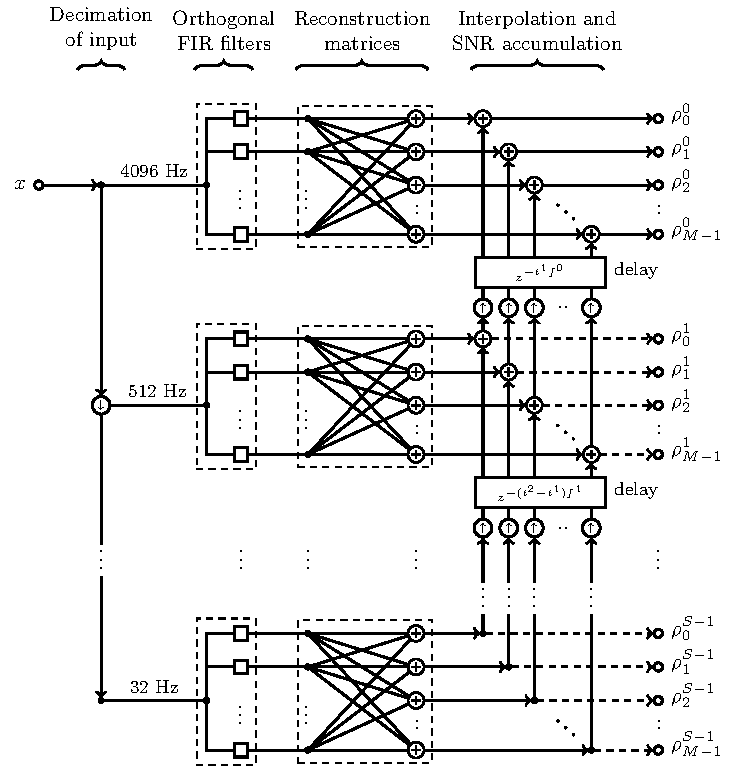
\includegraphics{figures/lloid-diagram.pdf}
		\caption{\label{fig:pipeline} Schematic of \lloid{} pipeline illustrating
signal flow.  Circles with arrows represent interpolation
\protect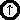
\includegraphics{figures/upsample-symbol.pdf} or decimation
\protect
\includegraphics{figures/downsample-symbol.pdf}.  Circles with plus
signs represent summing junctions
\protect
\includegraphics{figures/adder-symbol.pdf}.  Squares
\protect
\includegraphics{figures/fir-symbol.pdf} stand for \fir{} filters.  Sample
rate decreases from the top of the diagram to the bottom.  In this diagram each
time slice contains three \fir\ filters that are linearly combined to produce
four output channels.  In a typical pipeline the number of \fir\ filters is
much less than the number of output channels.}
	\end{center}
\end{figure*}
%
%
The signal flow diagram in figure~\ref{fig:pipeline} illustrates how this
recursion relation can be realized as a multi-rate filter network with outputs for
each of the early-warning \SNR{}s.

In the next section we compute the expected computational cost scaling of this
decomposition and compare it with the brute-force \TD{} implementation of
\eqref{eq:SNRTD} and higher latency \FD{} methods.

\subsection{Comparison of computational costs}

We now examine the computational cost scaling of the conventional \TD{} or
\FD{} matched filter procedure as compared with \lloid{}.  For convenience,
table~\ref{tab:recap} provides a review of the notation that we will need in
this section.
%
% symbols used in FLOPs calculations table
%
\begin{table}
\caption{\label{tab:recap}Notation used to describe filters.}
\begin{tabular}{ll}
\tableline\tableline
& Definition \\
\tableline
\numtmps		& num. of templates \\
\tmpsamps	& num. of samples per template \\
\numslices	& num. of time slices \\
\numsvdtmps	& num. of orthogonal templates in time slice $s$ \\
\slicessamps	& num. of samples in decimated time slice $s$\\
$f^s$		& sample rate in time slice $s$ \\
$N^\shortdownarrow$ & num. of coefficients in decimation filter \\
$N^\shortuparrow$ & num. of coefficients in interpolation filter \\
\tableline
\end{tabular}
\end{table}


\subsubsection{Conventional \TD{} method}

The conventional \TD{} method consists of a bank of \fir{} filters, or sliding-window dot products.  If there are $\numtmps$ templates, each $\tmpsamps$ samples in length, then each filter requires $M N$ multiplications and additions per sample, or $2 \numtmps \tmpsamps f^0$ floating point operations per second (\flops) at a sample rate $f^0$.

\subsubsection{Conventional \FD{} method}

The most common \FD{} method is known as the \emph{overlap-save} algorithm, described in \citep{numerical-recipes-chapter-13}.  It entails splitting the input into blocks of $D$ samples, $D > \tmpsamps$, each block overlapping the previous one by $D - \tmpsamps$ samples.  For each block, the algorithm computes the forward \fft\ of the data and the templates, multiplies them, and then computes the reverse \fft.

Modern implementations of the \fft, such as the ubiquitous \texttt{fftw}, require about $2 \fftblock \lg \fftblock$ operations to evaluate a real transform of size $\fftblock$~\citep{Johnson:2007p9654}.  Including the forward transform of the data and $M$ reverse transforms for all of the templates, the \fft\ costs $2 (\numtmps + 1) \fftblock \lg \fftblock$ operations per block.  The multiplication of the transforms adds a further $2 \numtmps \fftblock$ operations per block.  Since each block produces $\fftblock - \tmpsamps$ usable samples of output, the overlap-save method requires
$$
f^0 \cdot \frac{2 (\numtmps + 1) \lg \fftblock + 2 \numtmps}{1 - \tmpsamps/\fftblock} \; \mathrm{\flops} \,.
$$

\subsubsection{\lloid\ method}

For time slices $s$, the \lloid\ method requires $2 \slicessamps \numsvdtmps f^s$ \flops\ 
for evaluating the orthogonal filters, $2 \numtmps \numsvdtmps f^s$ \flops\ for the 
linear transformation from the $\numsvdtmps$ basis templates to the $\numtmps$ time-sliced templates, and $\numtmps f^s$ \flops\ to add the resultant partial \SNR\ stream.

The computational cost of the decimation of the detector data is a little bit more subtle.  Decimation is achieved by applying an \fir\ anti-aliasing filter and then down-sampling, or deleting samples in order to reduce the sample rate from $f^{s-1}$ to $f^s$.  Naively, an anti-aliasing filter with $N^\shortdownarrow$ coefficients should demand $2 N^\shortdownarrow f^{s-1}$ \flops.  However, it is necessary to evaluate the anti-aliasing filter only for the fraction $f^s / f^{s-1}$ of the samples that will not be deleted.  Consequently, an efficient decimator that requires only $2 N^\shortdownarrow f^{s-1} \cdot \left( f^s / f^{s-1} \right) = 2 N^\shortdownarrow f^s$ \flops\ is possible.

The story is similar for the interpolation filters used to change the sample rates of the partial \SNR{} streams.  Interpolation of a data stream from a sample rate $f^s$ to $f^{s-1}$ consists of inserting zeros between the samples of the original stream, and then applying a low-pass filter with $N^\shortdownarrow$ coefficients.  The low-pass filter requires $2 M N^\shortdownarrow f^{s-1}$ \flops.  However, by taking advantage of the fact that by construction a fraction $f^{s-1}/f$ of the samples are zero, it is possible to build an efficient interpolator that requires only $M N^\shortuparrow f^{s-1} \cdot \left( f^s / f^{s-1} \right) = 2 M N^\shortuparrow f^s$ \flops.

Taking into account the decimation of the detector data, the orthogonal \fir\ filters, the reconstruction of the time-sliced templates, the interpolation of \SNR\ from previous time slices, and the accumulation of \SNR, in total the \lloid\ algorithm requires
$$
\sum_{\mathclap{s=0}}^{\mathclap{S-1}} \left( 2 \slicessamps \numsvdtmps + 2 \numtmps \numsvdtmps + \numtmps \right) f^s + 2\sum_{\mathclap{f \in \{f^s\}}} \left( N^\shortdownarrow + \numtmps N^\shortuparrow \right)
$$
\flops.  The second sum is carried out over the set of distinct sample rates rather than over the time slices themselves.

